\documentclass[border=3pt,tikz]{standalone}
\usetikzlibrary{arrows}
\usetikzlibrary{positioning}
\usetikzlibrary{calc}
\usetikzlibrary{arrows}
\begin{document}
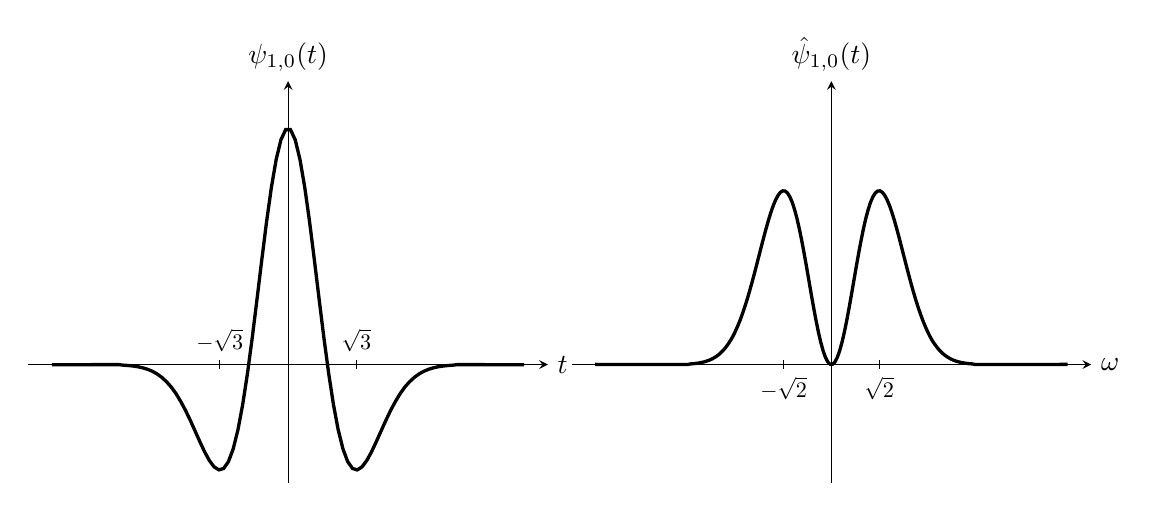
\begin{tikzpicture}[samples = 200, scale=3]

    \draw[-{stealth}] (-1.1, 0) -- (1.1,0) node[right] {$t$};
    \draw[-{stealth}] (0,-0.5) -- (0,1.2) node[above] {$\psi_{1, 0}(t)$};
    \draw[color=black, very thick, domain=-6:6, samples=100, variable = \t]   plot ({\t/6}, {(1-(\t)^2)*exp(-\t*\t/2)});
    \draw (-0.289, -0.02)-- (-0.289, 0.02) node[above, scale=0.8] {$-\sqrt{3}$};
    \draw (0.289, -0.02)-- (0.289, 0.02) node[above, scale=0.8] {$\sqrt{3}$};
    
    \begin{scope}[xshift=2.3cm] 
    
    \draw[-{stealth}] (-1.1, 0) -- (1.1,0) node[right] {$\omega$};
    \draw[-{stealth}] (0,-0.5) -- (0,1.2) node[above] {$\hat{\psi}_{1, 0} (t)$};
    
    \draw[color=black, very thick, domain=-7:7, samples=200, variable = \t]   plot ({\t/7}, {\t*\t*exp(-\t*\t/2)});
    
    \draw (-0.202, 0.02)-- (-0.202, -0.02) node[below, scale=0.8] {$-\sqrt{2}$};
    \draw (0.202, 0.02)-- (0.202, -0.02) node[below, scale=0.8] {$\sqrt{2}$};
    \end{scope}
    
    
    
    \end{tikzpicture}
\end{document}